\documentclass[a4paper]{arrowhead}

\usepackage[yyyymmdd]{datetime}
\usepackage{etoolbox}
\usepackage[utf8]{inputenc}
\usepackage{multirow}

\renewcommand{\dateseparator}{-}

%% Special references
\newcommand{\scref}[2]{{\textcolor{ArrowheadBlue}{\hyperref[sec:services:consumed:#1]{#2}}}}
\newcommand{\scdef}[2]{{\textcolor{ArrowheadBlue}{#2\label{sec:services:consumed:#1}}}}
\newcommand{\spref}[2]{{\textcolor{ArrowheadBlue}{\hyperref[sec:services:produced:#1]{#2}}}}
\newcommand{\spdef}[2]{{\textcolor{ArrowheadBlue}{#2\label{sec:services:produced:#1}}}}
%%

\begin{document}

%% Arrowhead Document Properties
\ArrowheadTitle{Event Handler}
\ArrowheadType{System Design Description}
\ArrowheadTypeShort{SysDD}
\ArrowheadVersion{4.3.0}
\ArrowheadDate{\today}
\ArrowheadAuthor{Szvetlin Tanyi}
\ArrowheadStatus{RELEASE}
\ArrowheadContact{szvetlin@aitia.ai}
\ArrowheadFooter{\href{www.arrowhead.eu}{www.arrowhead.eu}}
\ArrowheadSetup
%%

%% Front Page
\begin{center}
  \vspace*{1cm}
  \huge{\arrowtitle}

  \vspace*{0.2cm}
  \LARGE{\arrowtype}
  \vspace*{1cm}
  \vspace*{\fill}

  % Front Page Image
  %\includegraphics{figures/TODO}

  \vspace*{1cm}
  \vspace*{\fill}

  % Front Page Abstract
  \begin{abstract}
    This document describes the Event Handler core system of the Eclipse Arrowhead Framework. The purpose of Event Handler supporting core system is providing authorized publish-subscribe messaging system to the Eclipse Arrowhead Framework.
  \end{abstract}

  \vspace*{1cm}

  \scriptsize
  \begin{tabularx}{\textwidth}{l X}
    \raisebox{-0.5\height}{
\includegraphics[width=2cm]{figures/artemis_logo}} & {ARTEMIS Innovation Pilot Project: Arrowhead\newline
    THEME [SP1-JTI-ARTEMIS-2012-AIPP4 SP1-JTI-ARTEMIS-2012-AIPP6]\newline
    [Production and Energy System Automation Intelligent-Built environment and urban infrastructure for sustainable and friendly cities]}
  \end{tabularx}
  \vspace*{-0.2cm}
\end{center}
\newpage
%%

%% Table of Contents
\tableofcontents
\newpage
%%

\section{Overview}
\label{sec:overview}

This document describes the Eclipse Arrowhead  Event Handler system,
which exists to provide a secure publish-subscribe messaging system in a Eclipse Arrowhead Local Cloud (LC). Examples of such interactions is a consumer subscribing to some kind of Eclipse Arrowhead Event. 

The purpose of this System is therefore to allow:
\begin{itemize}
    \item Application systems to publish their event types.
    \item Consumers to subscribe and unsubscribe to events.
\end{itemize}


\section{System Role}
\label{sec:role}

\begin{figure}[t!]
  \centering
  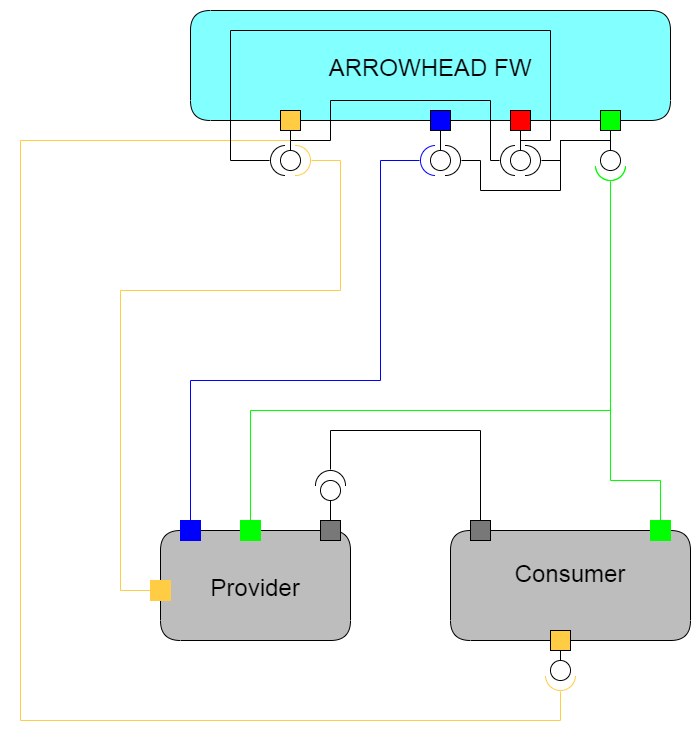
\includegraphics[width=0.8\textwidth]{figures/event_handler_overview.png}
  \caption{This diagram shows how consumers and providers are connected to the Arrowhead Framework and each other.}
  \label{fig:overview}  
\end{figure}

The color coding on Figure \ref{fig:overview} shows:

 \begin{itemize}
      \item Blue: Service Registry
      \item Red: Authorization
      \item Green: Orchestration
      \item Yellow: Event Handler
  \end{itemize}

This System provides multiple Core Services, \textbf{Echo}, \textbf{EventPublish}, \textbf{EventSubscribe}, \textbf{EventUnsubscribe}.


There are four use case scenarios connected to the Event Handler.
\begin{itemize}
    \item Event publishing
    \item Register subscription
    \item Unregister Subscription
\end{itemize}

The Event publish interface is used to o deliver Event to all relevant Subscribers. 

The register interface is used to register a subscription.

The unregister interface is used to unregister an subscription.

\section{Services}
\label{sec:services}


\subsection{Consumed Services}

\subsubsection{\spdef{CheckAuthorizationSubscription}{CheckAuthorizationSubscription}}

This service checks whether a given application system is allowed to receive events from another application system.

\subsubsection{\spdef{Notification}{Notification}}

This service is provided by the event consuming application system where the Event will be sent.


\subsection{Provided Services}

\subsubsection{\spdef{Echo}{Echo}}

This service allows to check the core systems availability.

\subsubsection{\spdef{EventPublish}{EventPublish}}

This service allows to application systems to publish events.

\subsubsection{\spdef{EventSubscribe}{EventSubscribe}}

This service allows application systems to subscribe to events.

\subsubsection{\spdef{EventUnsubscribe}{EventUnsubscribe}}

This service allows application systems to unsubscribe from events.

\section{Security}
\label{sec:security}

This System can be secured via the HTTPS protocol. If it is started in secure mode, it verifies whether the Application System possesses a proper X.509 identity certificate and whether that certificate is Arrowhead compliant in its' making. This certificate structure and creation guidelines ensure:

\begin{itemize}
    \item Application System is properly bootstrapped into the Local Cloud
    \item The Application System indeed belongs to this Local Cloud
    \item The Application System then automatically has the right to register its Services in the Registry.
   
\end{itemize}

 If these criteria are met, the Application System’s registration or removal message is processed. An Application System can only delete or alter entries that contain the Application System as the Service Provider in the entry.



\newpage

\bibliographystyle{IEEEtran}
\bibliography{bibliography}

\newpage

\section{Revision History}
\subsection{Amendments}

\noindent\begin{tabularx}{\textwidth}{| p{1cm} | p{3cm} | p{2cm} | X | p{4cm} |} \hline
\rowcolor{gray!33} No. & Date & Version & Subject of Amendments & Author \\ \hline

1 & 2020-12-05 & 4.3.0 &  & Tanyi Szvetlin \\ \hline


\end{tabularx}

\subsection{Quality Assurance}

\noindent\begin{tabularx}{\textwidth}{| p{1cm} | p{3cm} | p{2cm} | X |} \hline
\rowcolor{gray!33} No. & Date & Version & Approved by \\ \hline

1 & 2021-01-18 & 4.3.0 & Jerker Delsing \\ \hline

\end{tabularx}

\end{document}